\section{Estado del arte}
\label{ch:estado_arte}
\subsection{Introducción y alcance}
El presente estado del arte releva investigaciones académicas, productos comerciales y tendencias tecnológicas vinculadas con la integridad académica en evaluaciones digitales mediante trazabilidad de autoría, biometría conductual, análisis de interacción y detección de eventos atípicos. Además de describir los antecedentes de autenticación de estudiantes, busca identificar la brecha específica que justifica el desarrollo de ImprontIA: una solución que aporte información sobre la integridad de la interacción en exámenes digitales sin depender de supervisión audiovisual continua mediante cámara, audio o bloqueo exhaustivo del dispositivo.

A partir de la evolución reciente de la inteligencia artificial generativa, el problema de integridad académica dejó de limitarse a la suplantación humana o al uso de materiales no autorizados. Hoy también deben considerarse la asistencia algorítmica, el uso de modelos de lenguaje durante la producción de respuestas y la posible intervención de agentes de IA capaces de navegar interfaces, escribir, hacer clic, desplazarse por una página y completar tareas en nombre de una persona. En este contexto, el proyecto adopta una noción de integridad académica centrada en la trazabilidad del proceso de producción de la respuesta: no solo importa si el usuario autenticado es el estudiante, sino también si la sesión conserva señales de interacción compatibles con el proceso esperado de producción de una respuesta académica.

El estado del arte se organiza en tres ejes: investigación académica reciente sobre biometría conductual, trazabilidad de autoría y detección de eventos atípicos; soluciones comerciales de \textit{proctoring} y herramientas de seguridad frente a automatización; y contexto regional y normativo aplicable en Argentina y Latinoamérica.

\subsection{Investigación académica reciente}
\subsubsection{Dinámica de tipeo (\textit{keystroke dynamics}) y modelos profundos}
La dinámica de pulsaciones de teclado constituye una de las modalidades de biometría conductual más estudiadas para autenticación continua. Su ventaja principal es capturar señales de identidad durante una actividad natural del usuario: escribir. En el contexto de evaluaciones digitales esto resulta especialmente relevante porque muchas tareas académicas requieren redactar respuestas, resolver ejercicios escritos o interactuar con formularios.

TypeNet representa uno de los puntos de inflexión del campo. Acien et al. propusieron una arquitectura basada en redes LSTM siamesas evaluada sobre más de 136 millones de pulsaciones de aproximadamente 168.000 usuarios en teclado físico. El trabajo reporta una EER de 2,2\,\% en teclados físicos y 9,2\,\% en teclados táctiles, resultados que muestran la viabilidad de aplicar \textit{keystroke biometrics} a escala masiva en escenarios de texto libre~\parencite{Acien2022}.

TypeFormer profundiza esta línea mediante arquitecturas Transformer adaptadas a señales temporales de escritura móvil. \textcite{Stragapede2024} reportan una EER de 3,25\,\% utilizando solo cinco sesiones de enrolamiento de 50 pulsaciones cada una en la \textit{Aalto Mobile Keystroke Database}. Este resultado es relevante para ImprontIA porque los exámenes reales no siempre permiten recolectar largos historiales previos; los métodos que funcionan con bajo volumen de enrolamiento son especialmente pertinentes.

La principal conclusión de esta línea es que los modelos profundos permitieron superar limitaciones de enfoques clásicos, pero persisten desafíos de generalización entre dispositivos, tamaños de muestra, idiomas, contextos de escritura y condiciones emocionales o cognitivas del usuario. Entre las necesidades abiertas del campo figura, por lo tanto, la validación con datos locales obtenidos en condiciones reales de evaluación.

\subsubsection{Dinámica del mouse (\textit{mouse dynamics}), multimodalidad y autenticación continua}
El análisis de movimiento del cursor aporta una segunda capa de señales conductuales. A diferencia del teclado, el mouse o \textit{trackpad} permite observar trayectorias, velocidad, aceleración, pausas, clics, desplazamientos y patrones de navegación. Estas variables son útiles tanto para verificar identidad como para distinguir interacciones humanas de interacciones automatizadas.

\textcite{Yang2022} propusieron un método de autenticación basado en la combinación de \textit{keystroke dynamics} y \textit{mouse dynamics} en escenarios híbridos, utilizando características independientes de la aplicación. Esta orientación es relevante para ImprontIA porque una evaluación digital puede incluir preguntas de opción múltiple, desarrollo escrito, navegación entre consignas y selección de archivos.

\textcite{Ayeswarya2025} desarrollaron un sistema de autenticación continua con fusión multibiométrica sensible al contexto, que combina \textit{keystroke dynamics} y biometría de marcha mediante un algoritmo de \textit{scoring} contextual. Aunque la marcha no es una señal directamente aplicable a un examen de escritorio, el aporte metodológico es significativo: muestra que la fusión de señales mejora robustez, usabilidad y capacidad de adaptación a cambios de contexto.

La literatura sobre aprendizaje federado aplicada a biometría agrega una dimensión clave de privacidad. \textcite{Guo2024} revisan avances en reconocimiento biométrico federado y presentan el \textit{federated learning} como alternativa para entrenar modelos sin centralizar datos biométricos sensibles. Para ImprontIA, esta línea es relevante porque permite proyectar arquitecturas en las que la institución reduzca la exposición de datos conductuales crudos.

\subsubsection{Antecedentes directos en exámenes en línea}
Los antecedentes más cercanos a ImprontIA provienen de trabajos que aplican biometría conductual específicamente a la autenticación de estudiantes en evaluaciones en línea. \textcite{Stewart2011} investigaron \textit{keystroke dynamics} y estilometría para autenticar examinados en exámenes en línea, obteniendo resultados favorables sobre una muestra universitaria reducida.

\textcite{Monaco2013} extendieron esta línea en el contexto de evaluación de cursos en línea, combinando verificación biométrica conductual de identidad estudiantil y autenticación de autoría textual. Estos estudios funcionan como prueba conceptual directa de que el proceso de escritura durante una evaluación puede aportar evidencia de identidad. Sus principales limitaciones para ImprontIA son el tamaño muestral reducido, el contexto cultural y lingüístico distinto y la ausencia de una solución integral que combine teclado, mouse, navegación y análisis de asistencia algorítmica.

Estos antecedentes dejan abiertas la validación con muestras más amplias, en otros idiomas y contextos culturales, con dispositivos heterogéneos y bajo marcos normativos locales, y la integración de varias señales de interacción en una misma solución educativa.

\subsubsection{Fraude asistido por IA y análisis del proceso de escritura}
La incorporación de modelos de lenguaje generativo modificó el problema de fraude académico. Los detectores de texto generado por IA analizan principalmente el producto final, pero son vulnerables a edición humana, paráfrasis, traducción, mezcla de fuentes o asistencia parcial. Por ello, una línea emergente propone desplazar el foco desde el contenido final hacia el proceso de producción.

\textcite{Mehta2025} estudian la detección de deshonestidad académica asistida por LLM mediante \textit{keystroke dynamics}, y plantean que las señales de escritura pueden revelar diferencias entre producción humana autónoma y escritura asistida por modelos de lenguaje. \textcite{Akcapinar2025} explora una dirección complementaria mediante \textit{behavior analytics} en exámenes en línea, incorporando eventos como pérdida de foco, selección de texto, clic derecho y patrones de interacción durante la evaluación.

Estas investigaciones son recientes y deben tratarse como literatura emergente. Proponen no limitarse a estimar si un texto parece generado por IA, sino observar cómo se produjo: ritmos de escritura, pausas, secuencias de edición, pegado de texto, cambios de foco, interacción con la consigna y continuidad del comportamiento durante la sesión. En esa línea, la salida que se plantea es un conjunto de indicadores para una revisión académica posterior.

\subsubsection{Agentes de IA, automatización web y detección humano-agente}
La aparición de agentes de IA capaces de operar interfaces digitales amplía todavía más el alcance del problema. OpenAI presentó Operator como un agente que utiliza su propio navegador para realizar tareas en la web; su modelo subyacente, Computer-Using Agent, fue diseñado para interactuar con interfaces gráficas mediante percepción visual y acciones como hacer clic, escribir y desplazarse~\parencite{OpenAI2025Operator,OpenAI2025CUA}. Anthropic incorporó una capacidad similar en Claude Computer Use, que permite a los desarrolladores indicarle al modelo que mire una pantalla, mueva el cursor, haga clic y escriba texto~\parencite{Anthropic2024CU}.

En investigación, BrowserAgent propone agentes con acciones de navegación inspiradas en el comportamiento humano, ejecutadas directamente sobre páginas web mediante Playwright~\parencite{Zhang2025BrowserAgent}. Otros trabajos, como Mind the Web y ceLLMate, analizan los riesgos de seguridad de los agentes que usan navegadores, incluyendo \textit{prompt injection}, abuso de permisos y necesidad de \textit{sandboxing}~\parencite{Shapira2025MindWeb,Meng2025ceLLMate}.

Desde la perspectiva de detección, FP-Agent constituye una fuente especialmente relevante. Wang, Shafiq y Vekaria realizaron un estudio controlado con siete agentes de navegación y usuarios humanos, recolectando huellas de navegador y señales conductuales en un sitio instrumentado. El resultado central es que los \textit{fingerprints} de navegador por sí solos pueden tener poder discriminativo limitado, mientras que los \textit{fingerprints} conductuales ---tipeo, desplazamiento y comportamiento de mouse--- permiten distinguir agentes de humanos y agentes entre sí~\parencite{Wang2026FPAgent}.

Esta línea de trabajo amplía el problema desde la autenticación continua del estudiante hacia la integridad de la interacción, que incluye la posible intervención de agentes automatizados. Su detección explícita es una pregunta abierta del campo y excede el alcance de este proyecto (Capítulo~\ref{ch:requerimientos}).

\subsection{Soluciones comerciales y ecosistema competitivo}
\subsubsection{\textit{Proctoring} educativo}
El mercado de \textit{proctoring} educativo está dominado por soluciones que combinan autenticación inicial, monitoreo por cámara, grabación de pantalla, bloqueo de navegador, análisis de audio, detección de objetos o personas y revisión posterior de incidentes. Entre los actores globales se encuentran Proctorio, Honorlock, Respondus, ExamSoft, Meazure/ProctorU, PSI, Inspera, Proctortrack y Mettl~\parencite{Heinrich2025, Balash2021}.

SMOWL es uno de los actores con mayor presencia en el mercado hispanohablante. Su comunicación comercial enfatiza compatibilidad con LMS, verificación de identidad y monitoreo de comportamiento durante exámenes en línea~\parencite{SMOWL}. Sin embargo, el paradigma general del \textit{proctoring} continúa dependiendo en gran medida de señales audiovisuales o de control del entorno digital.

La literatura académica documenta tensiones relevantes en este enfoque. \textcite{Balash2021} muestran que los estudiantes expresan preocupación por la cantidad y naturaleza personal de la información compartida con empresas de \textit{proctoring}. \textcite{Mutimukwe2023} destacan principios como transparencia, minimización, consentimiento, seguridad y responsabilidad desde la perspectiva de la privacidad como integridad contextual. \textcite{Newton2024} advierten limitaciones metodológicas en la evidencia disponible sobre deshonestidad en línea y la necesidad de interpretarla con cuidado.

Esta tensión define el espacio en el que se ubica ImprontIA: las instituciones necesitan mecanismos de integridad, pero los sistemas basados en cámara, audio y vigilancia intensiva pueden generar resistencias, estrés, problemas de equidad y riesgos de privacidad~\parencite{Balash2021, Coghlan2021}.

\subsubsection{Biometría conductual aplicada a fraude e identidad}
El mercado de biometría conductual está más desarrollado en banca, \textit{fintech} y prevención de fraude que en educación. BioCatch es el referente global del segmento financiero. En Argentina, Banco Galicia, Naranja X y Santander Argentina anunciaron en mayo de 2025 su incorporación a BioCatch Trust Argentina, una red interbancaria basada en señales de comportamiento y dispositivo para prevención de fraude en tiempo real~\parencite{BioCatch2025Argentina}. La relevancia para ImprontIA es técnica, no sectorial: BioCatch valida comercialmente el uso de actividad de teclado, mouse, pantalla táctil y dispositivo como señales de riesgo.

La escala del mercado confirma madurez del segmento. Permira completó en septiembre de 2024 una posición mayoritaria en BioCatch a una valuación de USD 1.300 millones~\parencite{Permira2024}, y BioCatch informó en julio de 2025 ingresos recurrentes anuales (ARR, por su sigla en inglés) superiores a USD 160 millones~\parencite{BioCatch2025ARR}. Estos datos muestran que la biometría conductual ya es una categoría comercial consolidada para fraude digital, aunque todavía no se haya trasladado con igual profundidad al ámbito educativo.

TypingDNA es el competidor funcional más cercano al enfoque educativo de ImprontIA. Su producto se presenta como autenticación por biometría de tipeo y menciona explícitamente el caso de uso de prevenir fraude en exámenes en línea mediante autenticación estudiantil respetuosa de la privacidad~\parencite{TypingDNA}. Sin embargo, su propuesta pública se concentra en autenticación por escritura y no en una capa integral de integridad que combine teclado, mouse, navegación, asistencia de IA y contexto regulatorio local.

\subsubsection{Detección de bots, automatización y agentes de IA}
Un tercer ecosistema relevante es el de detección de bots, automatización y agentes de IA. Cloudflare introdujo AI Labyrinth como un mecanismo para ralentizar y desgastar \textit{crawlers} de IA que no respetan directivas de no rastreo~\parencite{Cloudflare2025}. DataDome propone una estrategia de \textit{Agent Trust Management} orientada a asegurar agentes de IA y reporta actividad creciente de \textit{crawlers} vinculados al ecosistema LLM~\parencite{DataDome2025}. HUMAN Security sostiene que el tráfico de agentes de IA puede detectarse mediante señales actualizadas y propone decisiones basadas en intención e impacto, no solo en origen~\parencite{HUMANSecurity2026}. Arkose Labs presenta Arkose Titan como plataforma para fraude humano, bots, \textit{scraping} y amenazas de IA agéntica~\parencite{ArksoseLabs}. Fingerprint comercializa señales de detección de bots basadas en inconsistencias de navegador, \textit{headless browsers}, herramientas de automatización y agentes de IA~\parencite{Fingerprint2026}.

Estos productos muestran que el mercado de seguridad web se está desplazando desde la detección de bots tradicionales hacia la gestión de tráfico automatizado inteligente. Sin embargo, su objetivo es proteger sitios, APIs, pagos o formularios; no evaluar el aprendizaje ni la autoría en un examen. Su traslado al ámbito educativo exigiría integrar las señales de automatización con criterios pedagógicos, revisión humana y garantías de debido proceso académico. La principal enseñanza de este ecosistema es metodológica: la detección moderna no puede depender de una única señal, sino combinar \textit{fingerprints} de dispositivo, señales conductuales, telemetría de sesión, contexto de tarea e indicadores de intención.

\subsubsection{Argentina y Latinoamérica}
En Argentina, el ecosistema de identidad digital se concentra en biometría fisiológica, especialmente reconocimiento facial, validación documental y prueba de vida. El Sistema de Identidad Digital (SID) de RENAPER permite validar identidad a distancia en tiempo real mediante biometría facial y fotografía del DNI~\parencite{RENAPER}. Nosis VID ofrece validación de identidad y detección de solicitudes fraudulentas en transacciones en línea~\parencite{Nosis}. Estas soluciones son relevantes para \textit{onboarding} o verificación inicial, pero no resuelven la continuidad de identidad durante un examen.

El mercado latinoamericano de \textit{proctoring} en línea muestra crecimiento, aunque con foco en soluciones tradicionales. Business Market Insights estimó el mercado regional en USD 24,46 millones en 2022 y proyectó USD 46,61 millones para 2028, con una tasa de crecimiento anual compuesta (CAGR) de 11,3\,\%~\parencite{BusinessMarketInsights}. Este dato sugiere demanda creciente por integridad en evaluación remota, pero no prueba la existencia de una solución regional centrada en biometría conductual pasiva.

Desde el punto de vista normativo, la Resolución AAIP N.\textsuperscript{o}~4/2019 adopta una definición de datos biométricos que incluye características conductuales de una persona humana que permitan o confirmen su identificación única~\parencite{AAIP2019Res4}. Esto ubica a \textit{keystroke dynamics}, \textit{mouse dynamics} y patrones de interacción dentro de un marco de protección de datos personales. En consecuencia, cualquier solución de este tipo queda sujeta a exigencias de consentimiento informado, minimización, finalidad específica, seguridad y retención limitada, a las que se suma la revisión humana de las alertas.

\subsection{Comparación de enfoques}
\begin{table}[h!]
    \caption{Comparación de enfoques existentes y posicionamiento de ImprontIA}
    \label{tab:comparacion_enfoques}
    \centering
    \small
    \begin{tabularx}{\textwidth}{p{2.4cm} p{2.8cm} p{2.4cm} p{2.3cm} p{3.2cm}}
        \toprule
        \tblhead \textbf{Enfoque} & \textbf{Ejemplos} & \textbf{Señales principales} & \textbf{Fortaleza} & \textbf{Limitación para ImprontIA} \\
        \midrule
        \textit{Proctoring} audiovisual
            & SMOWL, Proctorio, Honorlock, Respondus
            & Cámara, audio, pantalla, navegador
            & Cobertura del entorno
            & Tensiones de privacidad, fricción/estrés y posibles sesgos según la implementación \\
        \addlinespace[4pt]
        Biometría conductual educativa
            & TypingDNA; Stewart et al.; Monaco et al.
            & Tipeo y latencias
            & Autenticación pasiva
            & Cobertura parcial si solo usa teclado \\
        \addlinespace[4pt]
        Biometría conductual financiera
            & BioCatch
            & Mouse, teclado, dispositivo, sesión
            & Madurez comercial
            & No es educativo \\
        \addlinespace[4pt]
        Detección de bots y agentes
            & Cloudflare, DataDome, HUMAN, Arkose, Fingerprint
            & \textit{Fingerprinting}, telemetría, automatización
            & Detecta tráfico automatizado
            & No evalúa autoría ni aprendizaje \\
        \addlinespace[4pt]
        \textbf{ImprontIA}
            & Propuesta del proyecto
            & Tipeo, mouse, navegación, foco, edición, anomalías
            & Integra trazabilidad de autoría, consistencia de interacción y revisión humana de eventos atípicos
            & Requiere validación empírica, \textit{dataset} local y criterios institucionales claros para interpretar alertas \\
        \bottomrule
    \end{tabularx}
\end{table}

\subsection{Análisis competitivo}
\label{ch:competencias}

Esta sección posiciona a ImprontIA frente al \textit{proctoring} audiovisual y la biometría conductual educativa relevados en las secciones anteriores del estado del arte, mediante la estrategia del océano azul y sus dos herramientas: la \textbf{Matriz ERIC} (Eliminar, Reducir, Incrementar, Crear) y la \textbf{Curva de Valor}. El posicionamiento resultante es deliberadamente complementario, no sustitutivo: ImprontIA renuncia a la observación audiovisual del entorno físico para priorizar la amplitud de señales digitales, la explicabilidad y la revisión humana.

\subsubsection{Enfoque competitivo y base del análisis}

El análisis competitivo de ImprontIA parte de la comparación de referencia (\textit{benchmark}) desarrollada en el Estado del Arte (Tabla~\ref{tab:comparacion_enfoques}), y utiliza esa evidencia como base para explicitar una estrategia de diferenciación mediante la Matriz ERIC y la Curva de Valor.

ImprontIA se propone como una capa complementaria de trazabilidad del proceso de resolución basada en señales de interacción digital, contextualización, explicabilidad y revisión humana. Como renuncia deliberada, prescinde de la observación del entorno físico mediante cámara o micrófono, sin que esa renuncia implique una superioridad general en privacidad o invasividad: el \textit{User Research} (Capítulo~\ref{ch:user_research}) muestra que la percepción de invasividad no depende únicamente del mecanismo utilizado, sino también de qué se captura, con qué finalidad y bajo qué condiciones se comunica.

\subsubsection{Estrategia del océano azul}
\label{sec:oceano_azul}

La estrategia del océano azul distingue dos tipos de espacio de mercado~\parencite{KimMauborgne2005}. Los océanos rojos son las industrias existentes, con fronteras y reglas de competencia aceptadas, en las que las empresas compiten por una demanda dada mejorando los mismos atributos que sus rivales. Los océanos azules son espacios todavía no disputados, que se crean mediante innovación en valor: en lugar de elegir entre diferenciarse o reducir costos, se replantean los factores que la industria da por sentados, eliminando o reduciendo algunos e incrementando o creando otros, para ofrecer un valor distinto a quien decide y a quien usa el producto.

En la supervisión de evaluaciones digitales, el \textit{proctoring} audiovisual se comporta como un océano rojo: sus productos compiten por ofrecer más observación del entorno físico, más restricciones del entorno digital y más alertas automáticas (Sección~\ref{ch:estado_arte}). ImprontIA compite en un espacio distinto: la trazabilidad del proceso de resolución, la interpretación de los eventos según las reglas de cada evaluación, la explicabilidad de cada indicador y el panorama agregado para el docente. La Matriz ERIC (Sección~\ref{sec:eric}) explicita qué factores se eliminan, reducen, incrementan y crean, y la Curva de Valor (Sección~\ref{sec:curva_valor}) representa el perfil resultante frente a las alternativas. Este posicionamiento es una hipótesis estratégica: la existencia efectiva de ese espacio de mercado requiere validarse con instituciones y docentes.

\subsubsection{Matriz ERIC}
\label{sec:eric}

La Matriz ERIC (Eliminar, Reducir, Incrementar, Crear), herramienta de la estrategia del océano azul~\parencite{KimMauborgne2005}, sintetiza las prioridades y renuncias de la propuesta frente al \textit{proctoring} audiovisual y la biometría conductual educativa relevados en el estado del arte. El cuadrante Crear refiere a elementos incorporados dentro de la propuesta de valor de ImprontIA y no a afirmaciones de novedad mundial.

\begin{table}[h!]
    \caption{Matriz ERIC de ImprontIA}
    \label{tab:matriz_eric}
    \centering
    \small
    \begin{tabularx}{\textwidth}{X X}
        \toprule
        \rowcolor{accent!15}\textbf{ELIMINAR} & \textbf{REDUCIR} \\
        \midrule
        \begin{minipage}[t]{\linewidth}
        \begin{itemize}[leftmargin=1em]
            \item Captura audiovisual del entorno físico como parte de la propuesta de ImprontIA.
            \item Dependencia del bloqueo del navegador o de la interrupción automática como mecanismo central de control.
            \item Decisiones académicas automáticas derivadas directamente de señales o indicadores.
        \end{itemize}
        \end{minipage}
        &
        \begin{minipage}[t]{\linewidth}
        \begin{itemize}[leftmargin=1em]
            \item Dependencia de una única modalidad o señal para interpretar una sesión.
            \item Alcance de la recolección a las señales necesarias y previamente definidas para cada evaluación.
            \item Interferencia del mecanismo de supervisión sobre el desarrollo normal de la evaluación.
        \end{itemize}
        \end{minipage} \\
        \addlinespace[6pt]
        \rowcolor{accent!15}\textbf{INCREMENTAR} & \textbf{CREAR} \\
        \midrule
        \begin{minipage}[t]{\linewidth}
        \begin{itemize}[leftmargin=1em]
            \item Amplitud de señales de interacción digital utilizadas para comprender la sesión.
            \item Contextualización académica de las señales e indicadores.
            \item Explicabilidad y trazabilidad entre indicador y evidencia de origen.
            \item Centralidad de la revisión humana antes de una valoración académica.
        \end{itemize}
        \end{minipage}
        &
        \begin{minipage}[t]{\linewidth}
        \begin{itemize}[leftmargin=1em]
            \item Una capa complementaria de trazabilidad del proceso de resolución.
            \item Una lectura integrada de señales de interacción digital y contexto académico.
            \item Un flujo explícito indicador \texorpdfstring{$\rightarrow$}{->} revisión humana \texorpdfstring{$\rightarrow$}{->} validación adicional cuando corresponda.
        \end{itemize}
        \end{minipage} \\
        \bottomrule
    \end{tabularx}
\end{table}

\subsubsection{Curva de Valor}
\label{sec:curva_valor}

La Curva de Valor, trazada sobre el cuadro estratégico~\parencite{KimMauborgne2005}, compara \textit{proctoring} audiovisual, biometría conductual educativa e ImprontIA sobre cuatro factores para los que el \textit{benchmark} del estado del arte permite una comparación defendible. La codificación Bajo~=~1, Medio~=~2 y Alto~=~3 se emplea únicamente con fines de representación visual; los niveles representan énfasis relativo de cada enfoque según el \textit{benchmark} analizado y no métricas de desempeño, precisión o calidad.

\begin{figure}[h!]
    \centering
    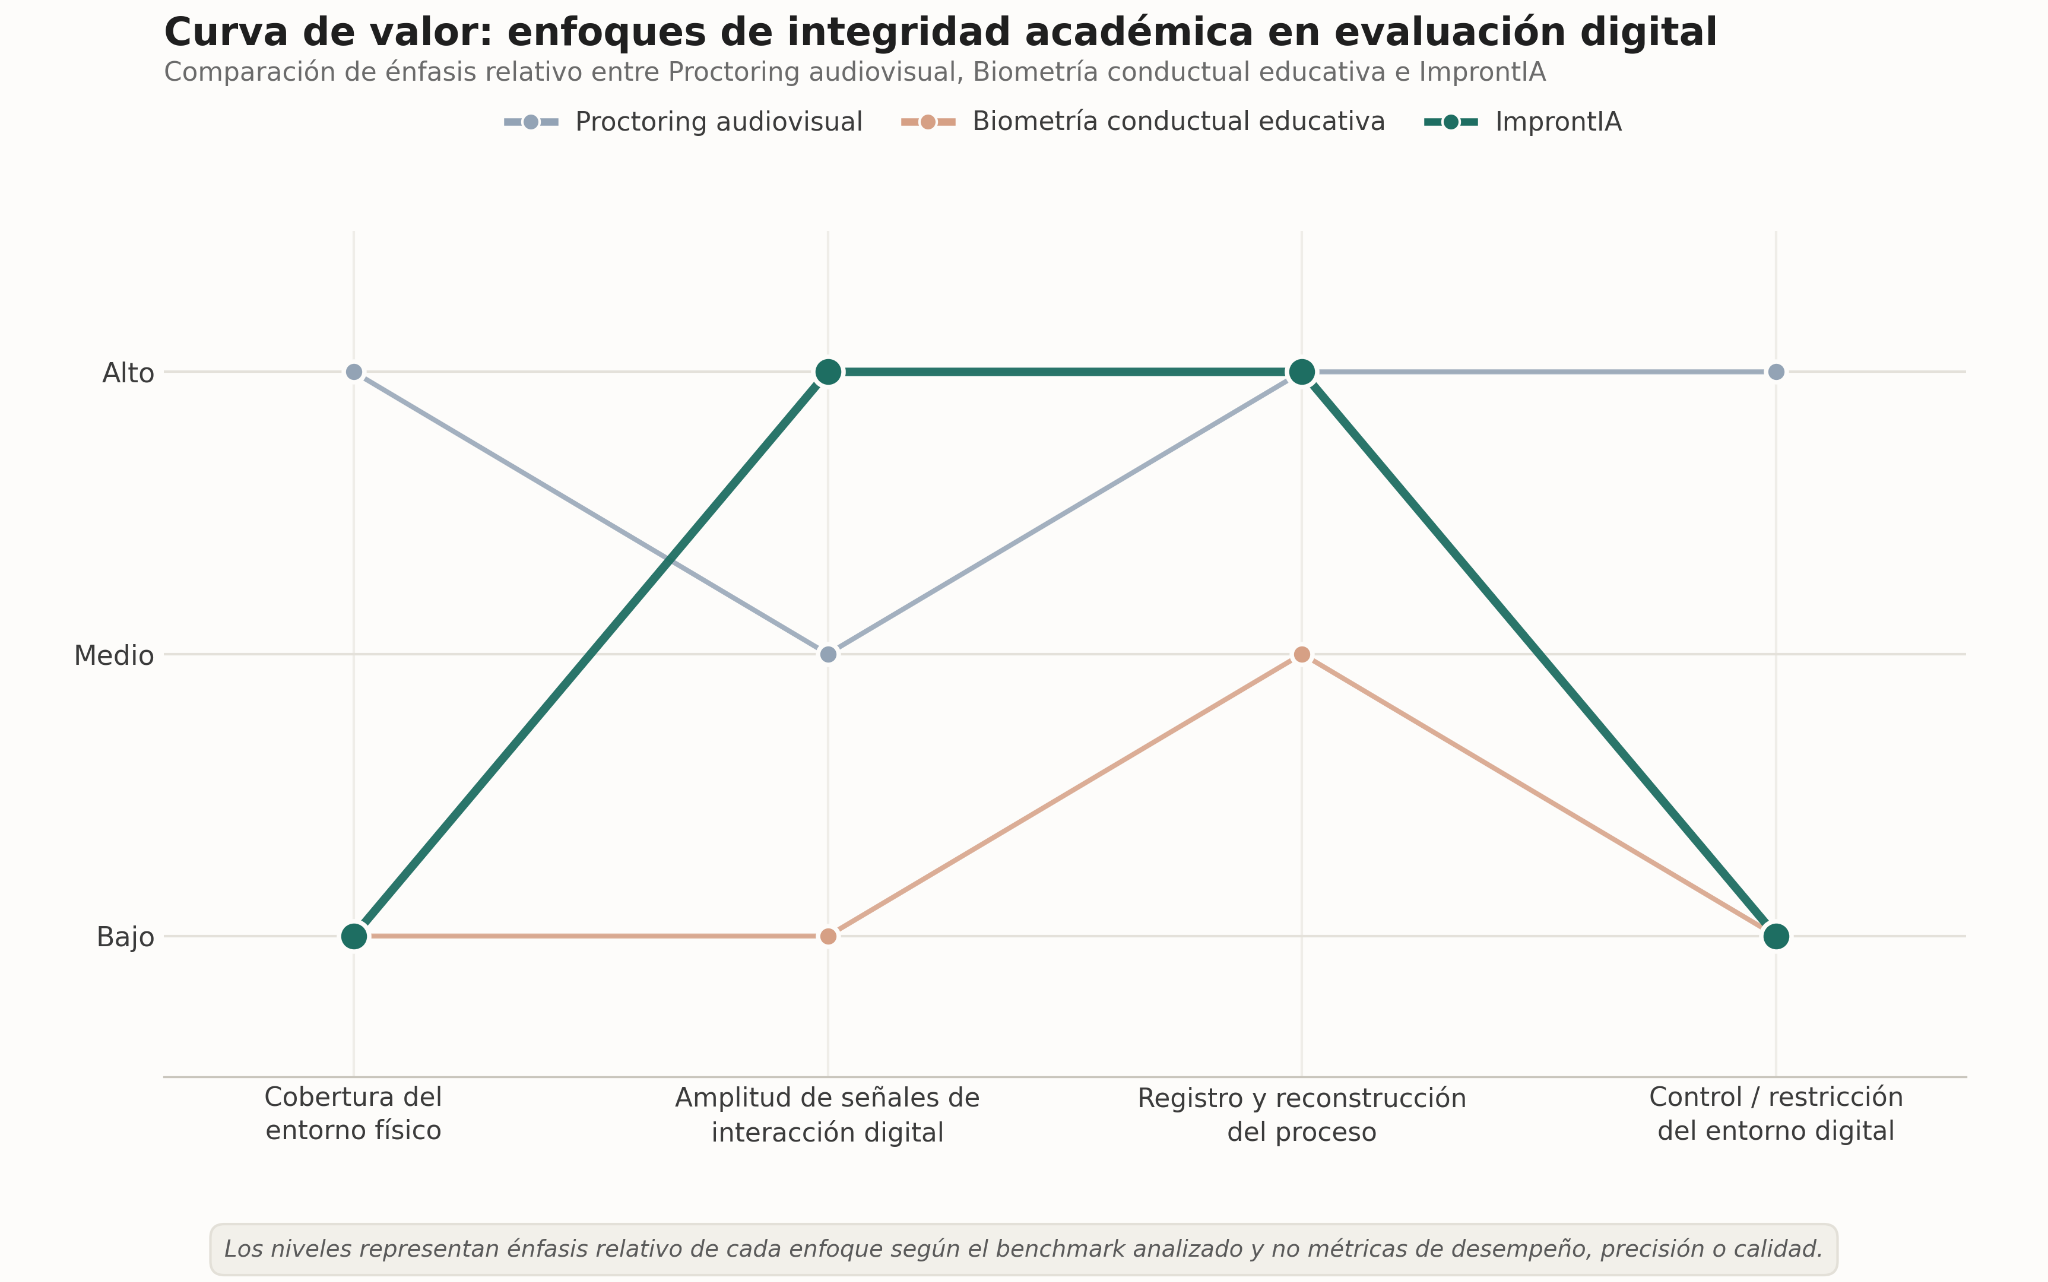
\includegraphics[width=0.95\textwidth]{./figures/competencias_curva_valor}
    \caption[Curva de Valor de ImprontIA frente a los enfoques comparados]{Curva de Valor de ImprontIA frente a los enfoques comparados. Fuente: elaboración propia a partir del \textit{benchmark} del estado del arte, sobre el cuadro estratégico de \textcite{KimMauborgne2005}.}
    \label{fig:curva_valor}
\end{figure}

\begin{table}[h!]
    \caption{Factores comparados en la Curva de Valor}
    \label{tab:curva_valor}
    \centering
    \small
    \begin{tabularx}{\textwidth}{X c c c}
        \toprule
        \tblhead \textbf{Factor} & \textbf{\textit{Proctoring} audiovisual} & \textbf{Biometría conductual educativa} & \textbf{ImprontIA} \\
        \midrule
        Cobertura del entorno físico & Alto (3) & Bajo (1) & Bajo (1) \\
        Amplitud de señales de interacción digital & Medio (2) & Bajo (1) & \textbf{Alto (3)} \\
        Registro y reconstrucción del proceso durante la sesión & Alto (3) & Medio (2) & \textbf{Alto (3)} \\
        Control / restricción del entorno digital & Alto (3) & Bajo (1) & Bajo (1) \\
        \bottomrule
    \end{tabularx}
\end{table}

\subsubsection{Síntesis de posicionamiento y renuncias}

La comparación muestra perfiles estratégicos diferentes y evita plantear una superioridad general de ImprontIA. El \textit{proctoring} audiovisual presenta mayor énfasis en la observación del entorno físico y en mecanismos de control o restricción del entorno digital, capacidades a las que ImprontIA renuncia deliberadamente. La biometría conductual educativa concentra su propuesta en un conjunto más acotado de señales, mientras que ImprontIA prioriza la amplitud de señales de interacción digital y la reconstrucción del proceso desarrollado durante la sesión.

Sobre esa base, ImprontIA incorpora como ejes de su propuesta la contextualización académica, la explicabilidad del vínculo entre indicadores y evidencia y la revisión humana. Estos factores no se incorporan a la Curva de Valor porque el \textit{benchmark} disponible no permite asignar niveles comparativos suficientemente rigurosos a las otras categorías en esas dimensiones.

\begin{keyfinding}{Posicionamiento resultante}
ImprontIA se posiciona como una capa \textbf{complementaria} ---no sustitutiva--- que aporta trazabilidad del proceso dentro del entorno digital, y mantiene separadas la generación de un indicador, la interpretación docente y una eventual validación adicional cuando corresponda.
\end{keyfinding}


\subsection{Brecha identificada y oportunidad para ImprontIA}
El relevamiento permite identificar una brecha clara. Por un lado, la investigación académica demuestra que la biometría conductual puede autenticar usuarios y detectar desviaciones en patrones de interacción. Por otro lado, el mercado educativo se apoya principalmente en \textit{proctoring} audiovisual, mientras que el mercado de biometría conductual se concentra en banca y fraude financiero. El mercado de detección de bots y agentes de IA desarrolla técnicas relevantes, pero orientadas a seguridad web general y no a evaluación académica.

En esa brecha se ubica ImprontIA, como una propuesta de integridad académica basada en el análisis pasivo de la interacción. Su diferenciación reside en la generación de señales revisables, y se apoya en dos preguntas complementarias: ¿la sesión mantiene patrones compatibles con la línea base esperada para esa evaluación (consistencia conductual)? y ¿el proceso de escritura y navegación muestra indicios de asistencia externa (autonomía de producción)? Una tercera pregunta que plantea la literatura reciente, si la secuencia de acciones corresponde a una persona o a un agente automatizado (humanidad de interacción), queda fuera del alcance del MVP, como se indicó al relevar esa línea de trabajo.

Esta formulación reemplaza la promesa técnicamente riesgosa de ``detectar fraude'' de manera concluyente por un planteo prudente: puntuación de anomalías, explicación de señales, trazabilidad, revisión humana y respeto por los principios de minimización de datos.

La oportunidad local también es significativa. No se identificó, en el relevamiento público disponible, una solución argentina o latinoamericana que combine biometría conductual pasiva, foco educativo, soporte para español y cumplimiento explícito del marco regulatorio argentino; la validación con datos universitarios locales y la detección de agentes de IA siguen siendo, además, necesidades abiertas del campo.

\subsection{Conclusión del estado del arte}
El estado del arte muestra que ImprontIA se ubica en una intersección poco cubierta entre integridad académica, biometría conductual, IA aplicada a detección de anomalías y seguridad frente a agentes automatizados. La literatura académica ofrece evidencia sólida sobre \textit{keystroke dynamics}, \textit{mouse dynamics} y autenticación continua; el mercado demuestra demanda creciente por soluciones de integridad y fraude; y la aparición de agentes de IA introduce una amenaza emergente que vuelve insuficiente el paradigma clásico de \textit{proctoring}.

La contribución esperada de ImprontIA es complementar las políticas institucionales de integridad académica priorizando señales de interacción digital que permitan identificar eventos o patrones atípicos para su revisión docente. Su valor diferencial reside en analizar el proceso de interacción ---cómo se escribe, se navega y se acciona--- en lugar de depender únicamente del contenido final, la cámara o la autenticación inicial; la proporcionalidad de cada señal debe analizarse según su naturaleza, su finalidad y el contexto de uso.

El principal desafío abierto del campo es validar empíricamente, con datos de usuarios reales, que las señales de interacción permiten distinguir, con niveles aceptables de error y explicabilidad, entre interacción genuina, suplantación, asistencia externa y automatización. La literatura revisada indica, además, que en un contexto universitario esa precisión técnica debe acompañarse de proporcionalidad, privacidad, transparencia y revisión humana. El posicionamiento de la propuesta frente a las alternativas relevadas se formalizó con la matriz ERIC y la curva de valor de la Sección~\ref{ch:competencias}, y su alcance concreto se delimita en los requerimientos del Capítulo~\ref{ch:requerimientos}.

La importancia del tema excede lo técnico: la confianza en las evaluaciones digitales condiciona la validez de las calificaciones y, en última instancia, de los títulos que emiten las instituciones, y las alternativas disponibles obligan hoy a elegir entre una vigilancia intensiva y la ausencia de información sobre el proceso. El aporte a la sociedad que busca el proyecto es una tercera vía: evidencia proporcionada al problema, reglas conocidas de antemano por el estudiante y decisiones siempre humanas. Sostener la confianza pública en la evaluación digital sin resignar la privacidad de quienes la rinden es, en ese sentido, una condición para que la expansión de la educación remota preserve su legitimidad.
